\chapter{Conflict Detection and Resolution System Architecture} % for Unmanned Aerial Vehicles in Civil Airspace}
\label{Ch:Architecture}

%\chapter{Introduction}
%\subchapter{Unmanned Aerial Vehicles and Their Integration into the Civil Airspace System}
\section{Introduction}
\lettrine[lines=3, nindent=0pt]{P}{rospective} applications of Unmanned Aerial Vehicles (UAV), or drones, have motivated many to commercially fly their UAVs in the civil airspace. This includes retail companies that want to offer a drone delivery service\footnotemark[1], media that want to obtain fast aerial footages\footnotemark[2], Internet companies that want to launch a high-altitude imagery drone\footnotemark[3], and countless other possibilities\cite{degarmo:04}. %, some of which depicted in Figure~\ref{f:Prospectives}\cite{degarmo:04}. 
These applications will only be commercially viable if UAV flights are integrated with, and are able to exploit fully the civil airspace. Currently, however, those flights are still considered to be strange and dangerous, and most authorities limit them to small secluded airspaces, commonly within operator line-of-sight\cite{CAP722}. 

One of the biggest concerns for UAV flights in the civil airspace is ensuring their operational safety in avoiding conflicts and collisions amongst themselves, as well as with the existing air traffic, especially when operated beyond line-of-sight. The public still has doubts about the operation, fearing that a vehicle might lose control at any time and might hit a person, building, or manned aircraft in proximity. What is lacking here is a general architecture that defines a Conflict Detection and Resolution (CD\&R) system, the particular system that handles the collision avoiding task in the airspace, that is versatile and safe enough to support UAV integration into the civil airspace. An exhaustive architecture should include methods for path-planning, separation assurance, and collision avoidance.
%
%\begin{figure}[h]
%	\centering
%	\includegraphics[width=1\linewidth]{Prospectives}
%	\caption{Prospective use of UAVs in Civil Airspace, adapted from Ref.~\cite{degarmo:04}}
%	\label{f:Prospectives}
%\end{figure}

Previous studies have resulted in various approaches for CD\&R systems for UAV, including both hardware and software concepts. Although these works show many promising results, the huge variation of approaches in literature leads to confusion on the integration management. Relying on only one choice of approach to handle every conflict situation will make the UAV vulnerable, since there would not be any back up system when failures occur. On the other hand, using several approaches from literature redundantly is not practical, since they might not exactly complement each other to be able to provide a general architecture for operation in the civilian airspace.

In comparison, manned-flight has managed to establish a multi-layered architecture of conflict detection and resolution by applying a fail-safe concept. Here, the architecture consists of several complementary approaches, commonly presented as `layers of safety'\cite{Dalamagkidis:09}, which includes from the outermost, (1) the Procedural, (2) the Air Traffic Management, (3) the Ground Surveillance, (4) the Cooperative, (5) the Coordinated, and (6) the `See and Avoid' Layer.% shown in Figure~\ref{f:MannedLayers}.
This kind of architecture was not formed instantly, but rather, it was built and iterated throughout the history of manned flight. Most of its components exist as the result of evaluations on accidents\cite{Kochenderfer:12}. A few examples of research that present such architectures for UAV CD\&R system are for example presented in Ref.~\cite{Yang:97}, Ref.~\cite{barfield:00},Ref.~\cite{Contarino01}, and Ref.~\cite{McCalmont:05}. One of the most comprehensive architecture designs can be found in the work in Ref. \cite{Graham:11}, which presents the Jointly Optimal Conflict Avoidance (JOCA). The problem of integration into the airspace, however, has not been thoroughly investigated nor has it been the driving factor in those designs.

% \begin{figure}[h]
% \centering
%  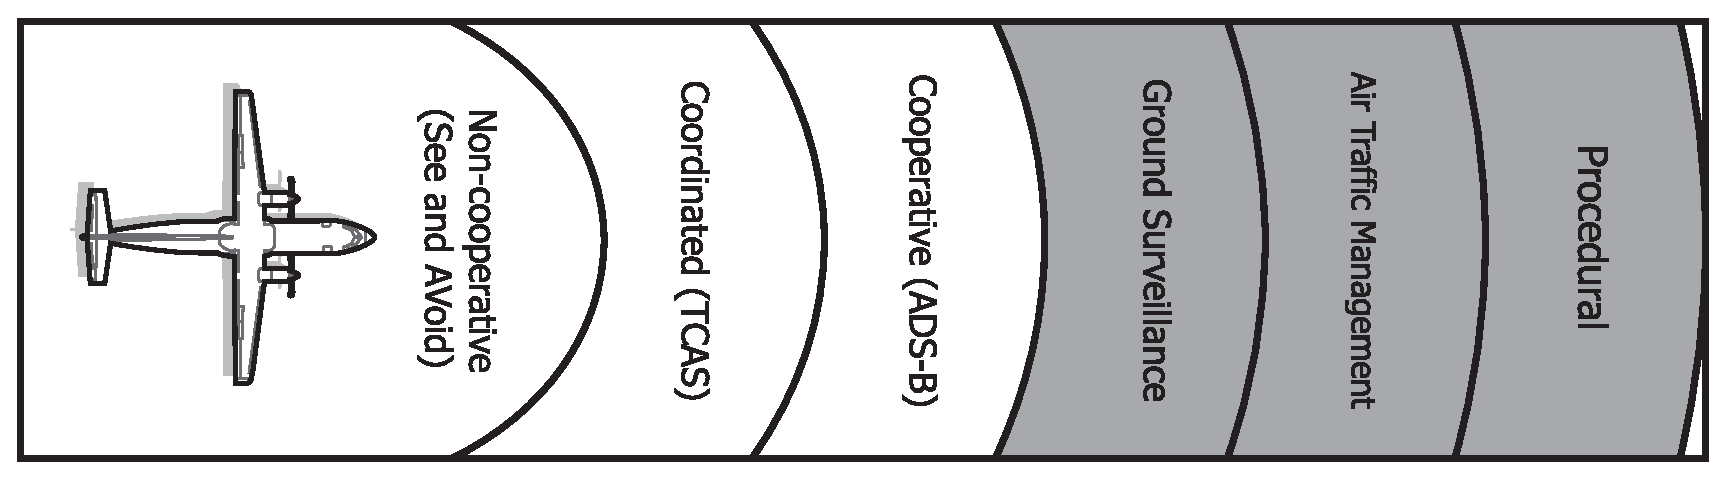
\includegraphics[width=10cm]{MannedLayers}
%  \caption{Layers of Safety from Manned-Flight, adapted from Ref.\cite{Dalamagkidis:09}}
%  \label{f:MannedLayers}
% \end{figure}
 % %put the new  sect in here

The current paper therefore proposes a novel architecture for a general UAV CD\&R system in the context of their integration into the civilian airspace. The proposed architecture is designed to manage various possible approaches in a complementary way, using the concept of a fail-safe system. The architecture is also designed to be practical guidelines for the authorities, operators, and developers, towards the integration of UAVs into the civil airspace. 
\footnotetext[1]{Gross, D., Amazon's Drone delivery: How would it work?" 2013, accessed September 2014, http://edition.cnn.com/2013/ 12/02/tech/innovation/amazon-drones-questions/}
\footnotetext[2]{Corcoran, M. "Drone journalism take off", 2012, accessed September 2014, http://www.abc.net.au/news/2012-02-21/drone-journalism-takes-off/3840616}
\footnotetext[3]{Gibbs, s. "Google’s Titan drones to take flight within months", 2015, accessed March 2015, http://www.theguardian.com/ technology/2015/mar/03/googles-titan-drones-to-take-flight-within-months}

Figure~\ref{f:CombinationPreview} shows the methodology applied in this paper to construct the architecture. Approaches to CD\&R, found in literature relating to both manned and unmanned systems, are broken down based on the choices in their method for (1) surveillance, (2) coordination, (3) maneuver, and (4) decision. This paper combines them back as generic approaches in succession, and reviews whether the resulting combination is appropriate or not, for the purpose of UAVs integration to the civil airspace. If it is appropriate, the process is continued until every choice of method is combined as a `\textit{generic approach}'. The resulting approaches are filtered one more time to remove redundancy. The final selection of appropriate approaches is then arranged to create the architecture of CD\&R for UAVs as a comprehensive fail-safe system.    

\begin{figure}[h!]
	\centering
	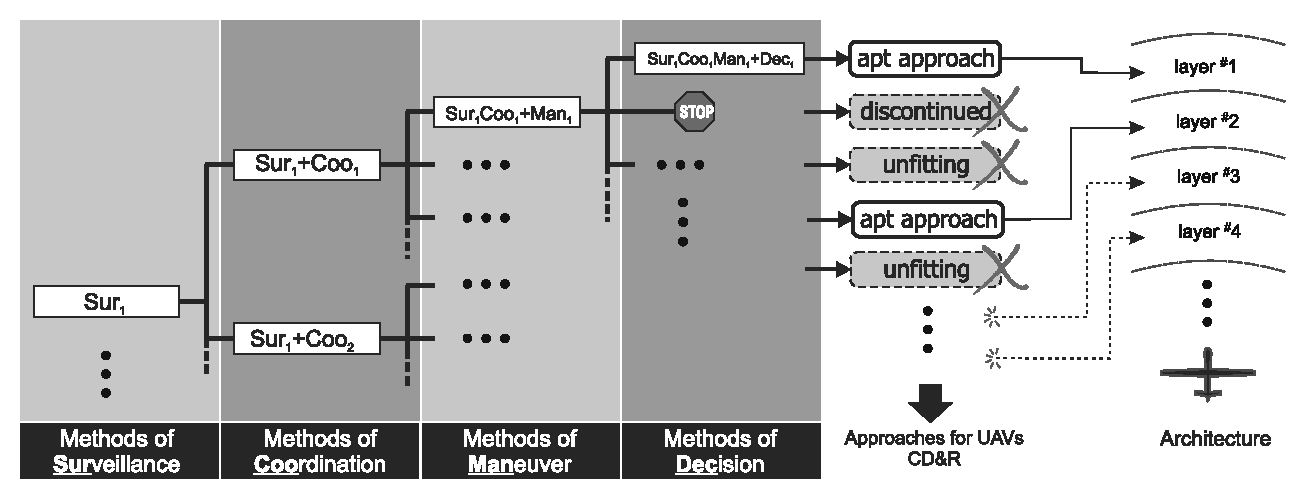
\includegraphics[width=0.9\linewidth]{\TheDir Figures/CombinationsPreview}
	\caption{Methodology in constructing the architecture of CD\&R for UAVs}
	\label{f:CombinationPreview}
\end{figure}

The research in this paper is presented as follows. After the introduction, Section 2 will elaborate on the existing approaches for the UAV CD\&R systems, breaking them down into four selections of methods. A taxonomy of CD\&R methods is presented in this section as well. Those methods are then combined back as generic approaches to CD\&R in the following Section 3, set as the components in building the architecture. This section also elaborates on why some of the existing approaches are not suitable in the context of UAV integration in the airspace. Section 4 presents a discussion of the general implementation of the architecture, along with few examples of prospective UAV operations\cite{degarmo:04}, including how the architecture affects the system and infrastructure requirements. Section 5 wraps the entire research in several conclusions and suggestions for future work. 


\section{Taxonomy of Methods for UAV Conflict Detection and Resolution} 

The UAV CD\&R approaches in the currently available literature are broken down and viewed as different combinations of choices for their method of surveillance, coordination, maneuver, and decision. For example, the Traffic Warning and Collision Avoidance System (TCAS) currently employed in manned aviation can be seen as a combination of \textit{distributed independent surveillance, explicit coordination, tactical maneuvering, and manual decision making}. These four properties  are presented in a taxonomy of CD\&R methods in Figure~\ref{f:Taxonomy}, in which they are arranged as four separated layers of safety. 

This research uses those four groups of methods, since they directly affect the airspace management once the UAVs are integrated. The surveillance and coordination might require cooperation from both other vehicle and local authorities. The maneuver type, depending on the portion of the changed path, might affect the global traffic. The choice of decision will define the role of the UAV operators. Other types of CD\&R taxonomies can also be found in the literature, such as in Ref.\cite{Kuchar:00}. However, they focus more on the internal algorithms that are not directly required for constructing the UAV CD\&R architecture, such as the state propagation, dimensions and resolutions.

\begin{figure}[h]
	\centering  
\includegraphics[width=0.6\textwidth]{\TheDir Figures/MethodsTaxonomy}
	\caption{Taxonomy of methods for UAV Conflict Detection and Resolution system}
	\label{f:Taxonomy}
\end{figure}

\subsection{Methods for the Airspace Surveillances}
Airspace surveillance is the first step in the CD\&R process, in which every possible conflicting object around the ownship should be detected. There are three types of surveillance that are currently used, shown in the taxonomy in Figure~\ref{f:Taxonomy}, which includes the following,

\begin{itemize}[labelindent=\parindent,leftmargin=5pc]
	\item[$\bullet$ \textbf{Sur}$_1:$] Centralized-dependent surveillance,
	\item[$\bullet$ \textbf{Sur}$_2:$] Distributed-dependent surveillance, and
	\item[$\bullet$ \textbf{Sur}$_3:$] Independent surveillance.
\end{itemize}

A centralized-dependent-surveillance system obtains data from a common station, or a station-network, and can be available even before the flight is conducted, e.g., a map of static obstacles. In manned-flight, this part is included in the first three layers, i.e., the Procedural, the Air Traffic Management, and the Ground Surveillance. The dominance in half of the layers shows the dependency of manned-flight on this type of surveillance. An aircraft can retrieve data about the traffic in an area, accompanied with the data about terrain and weather, from common ground centers like the Air Traffic Control (ATC) or the Aviation Weather Center (AWC). UAV operators are most likely to employ these data to plan each flight and avoid any unnecessary conflicts. An example of this practice is demonstrated in Ref.~\cite{Nikolos:03} and Ref.~\cite{Brooker:13}. 

A distributed-dependent-surveillance system obtains data from the traffic itself. This surveillance method, therefore, requires cooperation from every vehicle to broadcast their flight data among each other. In manned-flight, this practice is conducted in the Cooperative and Coordinated layers, by using the Automatic Dependent Surveillance Broadcast (ADS-B)\cite{McCallie:11} system, and the Traffic Warning and Collision Avoidance System (TCAS), respectively.  Applications for UAVs have been made for both of those systems, such as presented in Ref.~\cite{Park:08} and Ref.~\cite{Zeitlin:07}, respectively. Furthermore, several works in literature that focus on obstacles within a certain threshold without specifically mentioning a surveillance method are considered to be using the distributed-dependent-surveillance system as well.

The third method of surveillance considers obtaining airspace data independently using an on-board sensor system. In manned-flight, this type of independent surveillance is only present through (human) visual confirmation, used in the last layer of safety, the `see and avoid' procedure\cite{FAR:91}. While in manned-flight this type seems to be the primordial system for avoidance, in the UAV domain it dominates most of the research, and as such, on-board sensors are the most popular way to provide surveillance in UAV studies. Various sensors has been assessed, including cameras (visual light and infra-red)\cite{Fasano:08}, acoustic sensors\cite{Muller:14}, acoustic-vector sensors\cite{Tijs:10}, and even miniaturized versions of active-sensors like the laser-range-finder\cite{Hrabar:11} or RADAR\cite{Moses:14}. 

These three types of surveillance methods are arranged in the first set of layers shown in Figure~\ref{f:Taxonomy}. The centralized-dependent-surveillance is placed as the outermost layer, since it is available even before a flight is conducted. In fact, for UAVs, centralized surveillances might only be suitable before flight, due to two reasons. Firstly, UAVs are commonly manufactured with a light non-metal material that is hard to detect by a ground station. Secondly, even if it can be detected, the prospective UAVs\cite{degarmo:04} are commonly designed to exploit the airspace without being limited by the predefined airways used in manned-flight. Therefore, most of the time the UAV will fly in an area that is not covered by ATC or any other common ground station. The distributed-dependent-surveillance follows as the middle layer, as it is available in-flight in a generally longer range than any independent-surveillance method. The surveillance, however, is available only when the vehicle is close enough to others that share their flight data. The innermost layer, therefore, is the independent surveillance system that should be available when the two other fail to prevent obstacles from coming closer.

\subsection{Methods for the Avoidance Coordination}
In order to simplify the calculation for resolution, many studies assume some level of coordination between the vehicles. This research differentiates the levels into three methods of coordination, as shown in the taxonomy, i.e., 
\begin{itemize}[labelindent=\parindent,leftmargin=5pc]
	\item[$\bullet$ \textbf{Coo}$_1:$] Explicitly coordinated avoidance,
	\item[$\bullet$ \textbf{Coo}$_2:$] Implicitly coordinated avoidance, and
	\item[$\bullet$ \textbf{Coo}$_3:$] Uncoordinated avoidance.
\end{itemize}

Avoidance is said to be explicitly coordinated if an explicit communication for confirmation exists among the involved vehicles. Hence, a specific resolution, often using a common algorithm, can be produced for each conflicting vehicle. Combination with a decider like a ground station is a common practice in manned-flight management, such as ATC or TCAS, which gives a pair of aircraft a confirmed advisory to avoid conflict. The ACAS Xu\cite{Kochenderfer:12}, the next generation of TCAS for UAV, on the other hand, shows an example of the explicit coordination in UAV avoidance. In this paper, collision avoidance algorithms that are intended to avoid static obstacles are also considered to be explicitly coordinated.

An avoidance is implicitly coordinated if each involved vehicles follows a common set of rules or strategies in their avoidance, which ensures coordination without the need for communicating resolution decisions. In other words, instead of using an explicit communication for confirmation, each vehicle assumes that the other will act according to the rules. Being partially limited by the rules, the vehicles will still have some level of freedom in their avoidance. This practice can actually simplify the resolution calculation by limiting the maneuver based on the encounter geometry, or setting up priorities based on vehicle types. An example of this type of coordination in manned-flight is the use of right-of-way rules in the `see and avoid' procedure\cite{FAR:91}. This set of rules distributes the right-of-way to the conflicting vehicle that results in, for example, some aircraft which can maintain their path while others conduct avoidance in a way the pilot sees fit\cite{FAR:91}. The 'Free-flight' concept introduced in Ref.~\cite{Hoekstra:01} and \cite{Hoekstra:02} is also an implicitly coordinated method for avoidance. The work in Ref.~\cite{LeTallec:05} and \cite{Jenie:13b} presents an example of this type of coordination for UAV applications. Furthermore, conflict resolution methods with assumption of non-maneuvering obstacles are included as a implicitly-coordinated avoidance.

When the avoidance is uncoordinated, each involved vehicle has their own preferences for resolution based on the conflict situation, without limitation from any rules. The ownship in this case assumes that the obstacle is rogue and may conduct unexpected maneuvers. This actually makes the resolution calculation difficult since it has to take into account every possible vehicle movement and collision risks from the conflict situation. In manned flight, this avoidance is not implemented except possibly in an acrobatic performance, or in a highly unlikely emergency situation, depending on the pilot judgment. In UAVs, some examples exist in UAVs with high maneuverability, such as presented in Ref.~\cite{Teo:04}. Some work, such as in Ref.~\cite{Winder:99}, applies this type by using a predefined set of actions for an aggressive sure-escape that avoids the entire portion of the risk at once.

The order of this group of method is shown in the taxonomy in Figure~\ref{f:Taxonomy}. The most preferable by both the operator and authorities is the avoidance that is explicitly-coordinated. As also true in manned-flight CD\&R procedure, this coordination should always be the first choice to avoid in any regulated flight. Furthermore, as the first choice, this coordination should have the longest range and time for avoidance, which is necessary for confirmation between the involved vehicles. When counterparts avoidances cannot be confirmed, the implicit coordination is applied next. This method can provide some situational prediction for a vehicle to act early enough during the communication failure. The uncoordinated avoidance is in the last place, and should be the last choice in avoidance, when any coordination fails to prevent obstacles intrusion. Compared with the coordinated, an uncoordinated avoidance can have both longer and shorter range. If the vehicle only uses a simple predefined automatic action, regardless the obstacle dynamics, then only a short range is required. However, if the resolution involves series of predictions to take into account every possible risk with limited information about the obstacle dynamic, then a longer processing time, as well as longer distance, is required. Since it should be the last choice, the method for resolving an uncoordinated avoidance should be fast enough in a limited available range.

\subsection{Methods for the Avoidance Maneuver}
As airborne vehicles, UAVs are able to perform many kinds of maneuver in the 3-Dimensional space. This research differentiates between three types of maneuver, as shown in Figure~\ref{f:Taxonomy} which includes,
 
\begin{itemize}[labelindent=\parindent,leftmargin=5pc]
	\item[$\bullet$ \textbf{Man}$_1:$] Strategic maneuver, % Flight Path Vector (FPV) change maneuver,
	\item[$\bullet$ \textbf{Man}$_2:$] Tactical maneuver, and %Deconflict maneuver, and
	\item[$\bullet$ \textbf{Man}$_3:$] Escape maneuver.
\end{itemize}

A strategic maneuver is a long-range action that changes the initial path flight-plan significantly, in the attempt to avoid possible traffic. The path change commonly generates several new waypoints to follow, where the change can be both vertical and horizontal. The flight-planning in manned flight, as well as the approval from the ATC for a change, is assumed to be included in this method for maneuver. The path-planning method, largely used in UAVs, is also included as a strategic maneuver, as can be found in Ref.~\cite{Nikolos:03} and \cite{Borrelli:06}.

A tactical maneuver is a medium range action that changes a small part of the flight path aiming to keep any deviation as small as possible. This type of maneuver focuses on ensuring a certain separation threshold reactively for the most imminent obstacle. The example of this method in manned-flight is the Airborne Separation Assurance System (ASAS), such as presented in Ref.~\cite{Ellerbroek:11}. Most of the advanced methods in collision avoidance system for UAV are using this maneuver as they maintain a small path deviation by using, for instance, geometric guidance\cite{Mujumdar:11} or a cost function\cite{Patel:11}. Several papers mention this type of maneuver as a deconflict maneuver\cite{barfield:00,Jenie:13a}.

The last approach is to escape any potential collision all together and conduct a maneuver solely to bring the vehicle to safety. The escape maneuver should be aggressive and conducted immediately, commonly using an open-loop command, driven by the maximum performance limit of the vehicle. While the other two methods bring the vehicle back to its mission in the end, this maneuver has an option to abort the original mission. In manned-flight, this type of maneuver is applied in the `see and avoid' layer, in the way that they ignore any optimization, and focus only on the safety. The way the TCAS and the ACAS X\cite{Kochenderfer:12} works, which follows a resolution advisory in relatively short distance, are also included as an escape maneuver. In UAV domain, several examples use this maneuver type, for example in Ref.~\cite{Bouabdallah:07} and in Ref.~\cite{Beyeler:09}.

The arrangement of this group, as shown in Figure~\ref{f:Taxonomy} is based on the portion of the flight path that is altered and, therefore, the distance required to conduct an avoidance. The strategic maneuver is placed as the outermost layer due to the large portion of flight path it changes. A tactical maneuver follows as the middle layer since it changes a smaller part of the flight path, but still requires some distance to accommodate the optimization process. This maneuver is used not only when the previous fails, but also when the change of waypoints strategically is not desirable since it will obstruct the mission of the vehicle. Escape is placed as the innermost layer as it is most likely to be applied as the last resort of avoidance that neglects the initial flight path all together.

\subsection{Methods for the Avoidance Decision}
Based on how the decision is made, UAVs can conduct a avoidance either with
\begin{itemize}[labelindent=\parindent,leftmargin=5pc]
	\item[$\bullet$ \textbf{Dec}$_1:$] Manual decision, or
	\item[$\bullet$ \textbf{Dec}$_2:$] Autonomous decision.
\end{itemize}

In this research, the methods are differentiated more on the source of the final decision, and not on the calculation process. For instance, if a vehicle calculates a conflict situation on-board, but then sends the results to the ground operator to decide, it is still considered to be  avoidance. Manual avoidance is preferable by most of the current UAV regulations, which limit their operation to within line-of-sight of the operator\cite{CAP722}. Beyond line-of-sight, however, the effectiveness of manual avoidance is greatly reduced, as the situational awareness of the operator becomes low, as also mentioned as a concern in Ref.~\cite{LeTallec:05}. In this case, the role of the operator should be changed to be a flight manager, rather than pilot. The decision for conflict avoidance, hence, should be given to the autonomous system on-board.

The autonomous decision-making process can consider many parameters at once in order to choose the best avoidance from a set of options, commonly for within a short period with insignificant nuisance to the operator. Currently, even though many studies proposed various methods, such as in Ref.~\cite{Huang:14}, this type of decision is not applicable in a commercial manned-flight due to safety reasons. Research in the UAV domain, on the other hand, has been focused mostly on the autonomous avoidance ability, since it provides better situational awareness and time-to-react. 

The arrangement in this group of methods is shown in the fourth set of layers in Figure~\ref{f:Taxonomy}. The manual approach is placed as the outer layer that acts as the first means of avoidance, which is available in the first phase of the flight. The autonomous decision, therefore, is placed in the inner layer, since it is most likely to be use beyond the line of sight where manual decision is difficult to make. In some situations, however, the manual decision might be preferable for the last layer before collision. For example, in cases when there exist a known failure on the vehicle on-board system or for evasive set of actions after a collision. Manual avoidance might even become a requirement for the last line of defense, considering that the operator should have the most final decision to ensure safety and overwrite any other avoidance. Therefore, no actual order is applied for these two methods of decision.

\section{Building the Architecture of Conflict Detection and Resolution}
The architecture is built by arranging possible approaches, which are generated by combining methods in the taxonomy. Using direct combination, there can be 54 possible generic approaches ($3$ methods-of-surveillance$\times 3$ methods-of-coordination$\times 3$ methods-of-maneuver$\times 2$ methods-of-decision).  Several of the combinations, however, will be unfeasible for the purpose of UAV integration into civil airspace, which means that not all of the 54 approaches can be used. In order to eliminate unfeasible combinations, the methods are combined in succession: one-by-one. In every step, each combination is tested whether it is appropriate for UAVs and the conditions when they are integrated into the civil airspace. This process is shown in Figure~\ref{f:Combination}, and is explained thoroughly in the following subsections. The resulting appropriate approaches are then arranged as the UAV layers of safety, following the concept of a fail-safe system. 

\subsection{Combination of Methods and Eliminations}

Figure~\ref{f:Combination} shows the whole combination process. Combinations that `survive' until the end are defined as appropriate approaches for applications on UAVs, especially in the context of integration into the airspace system. The selection process combines methods from each group with methods in the other groups one-by-one, starting from the surveillance methods and ending with the avoidance decision. Some combinations, however, are discontinued due to their incompatibility with UAV applications or because they do not fit within the context of airspace integration. This elimination processes is elaborated in the following subsections.

\begin{figure}[t!]
 \centering
  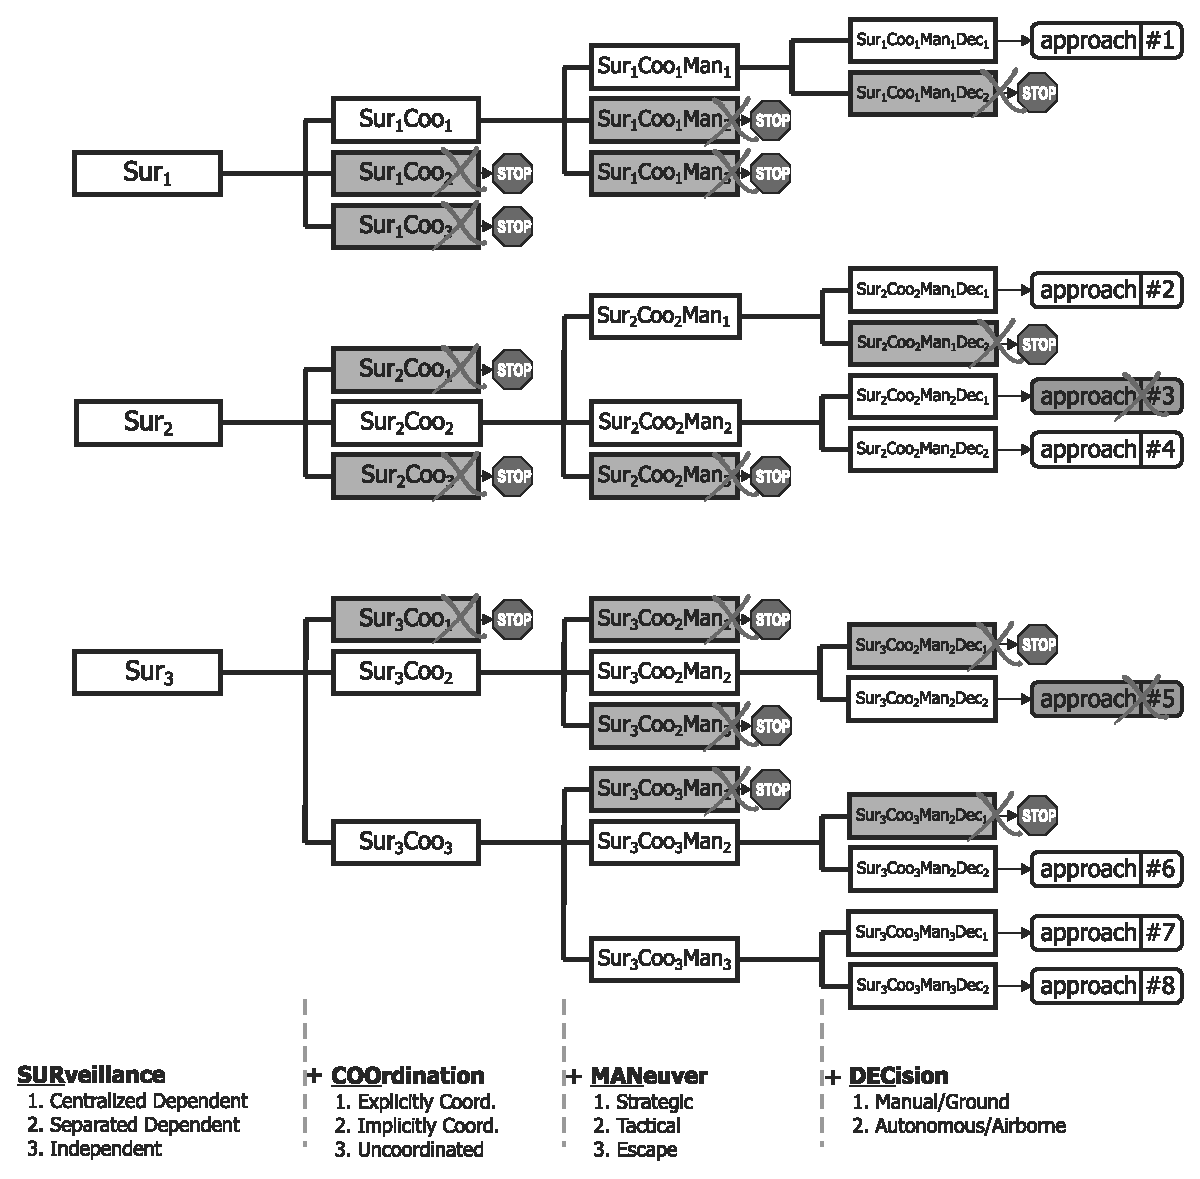
\includegraphics[width=0.95\textwidth]{\TheDir Figures/Combinations}
  \caption{Combination and elimination process of the methods of Surveillance, Coordination, Action, and Decision}
  \label{f:Combination}
\end{figure}
 
 \subsubsection{Combination of the Methods for Surveillance and Coordination}
As shown in Figure~\ref{f:Combination}, not all combinations of surveillance and coordination methods are accepted. There are four combinations that are eliminated due to the following reasons. The centralized-dependent-surveillance cannot support an implicitly coordinated (\textbf{Sur$_1$Coo$_2$}) or an uncoordinated avoidance (\textbf{Sur$_1$Coo$_3$}). These two types of coordination are most likely to be conducted when airborne, while the centralized surveillance for UAVs is only applied before the flight is conducted, as explained in section IIA. Using distributed-dependent surveillance for explicit coordination (\textbf{Sur$_2$Coo$_1$}) is also unfeasible, since it would require each UAV to have the same system, like the TCAS in manned flight. Assuming that once they are integrated, UAVs will vary wildly in type and size, it would be impractical to enforce all of them to carry the same system with the same algorithm for conflict resolution. The surveillance combination with uncoordinated avoidance (\textbf{Sur$_2$Coo$_3$}), furthermore, is also discontinued. The reason is that if every vehicle cooperatively shares their flight-data, it would be a waste to act without some sort of coordination. Lastly, the independent surveillance obviously cannot be used to support an explicit coordination (\textbf{Sur$_3$Coo$_1$}), since there is no communication between vehicles. 

 \subsubsection{Combination with the Methods for Maneuver}
The combination process is then continued with the methods of maneuver, as shown by the third column of Figure~\ref{f:Combination}. There are twelve possible combinations that can result from this process, of which six are discontinued. Similar to the coordination methods, the second and third row of combinations (\textbf{Sur$_1$Coo$_1$Act$_2$}) and (\textbf{Sur$_1$Coo$_1$Act$_3$}) are eliminated, since the centralized-dependent-surveillance can neither support tactical nor escape maneuvers, due to its preflight/ground only applicability. 

The distributed-dependent surveillance could actually support all three types of maneuver. The combination with the escape maneuver(\textbf{Sur$_2$Coo$_2$Act$_3$}), however, is unnecessary, considering the range covered by the surveillance and the cooperative nature of the involved aircraft. 

Combining the independent-surveillance with an implicitly coordinated avoidance can only be realized with a tactical maneuver. Asking the other UAV to change its strategically planned waypoints, in order to follow the implicit coordination (\textbf{Sur$_3$Coo$_2$Act$_1$}), is probably too much. The same reasoning is used in the elimination of the implicitly coordinated escape maneuver, (\textbf{Sur$_3$Coo$_2$Act$_3$}); an ownship cannot always expect the counterpart to do an aggressive escape maneuver. 

The support of independent-surveillance for an uncoordinated avoidance can be realized using either a tactical or an escape maneuver. The former is a popular method use in many studies that aim to conduct the most efficient UAV uncoordinated avoidance, based on on-board sensors. The latter is usually the solution for fast avoidance to safety whenever there is only limited information available on the conflict. The combination with strategic maneuvers (\textbf{Sur$_3$Coo$_3$Act$_1$}), however, is not suitable; an independent-surveillance generally has too short of a detection range to conduct a significant change in flight path.

 \subsubsection{Combination with the Methods of Decision}
The fourth and final column of Figure~\ref{f:Combination} represents the combination process with the methods of decision, whether it is made manual or autonomous. From the remaining six, twelve more methods can be produced in this level. 

The elimination starts with the consideration that a strategic maneuver should be conducted manually, due to the large portion of the path that will be changed. Therefore, two of the autonomous combinations, (\textbf{Sur$_1$Coo$_1$Act$_1$Dec$_2$} and \textbf{Sur$_2$Coo$_2$Act$_1$Dec$_2$}), are eliminated. The decision to avoid tactically, on the other hand, can be made both manually and autonomously. If it is supported by an independent-surveillance (\textbf{Sur$_3$Coo$_2$Act$_2$Dec$_1$}), the situational awareness at ground will not be sufficient and, hence, eliminated. Moreover, even if the independent-surveillance is accurate enough, the detection range is already too close for the ground operator to process the exchanged data. Therefore, the manual avoidance is eliminated (\textbf{Sur$_3$Coo$_3$Act$_2$Dec$_1$}) in the independent surveillance group.

The last combination in the fourth column of Figure~\ref{f:Combination}, however, actually presents a manual escape maneuver that is supported by an independent surveillance. This is a special case of escape in a situation where the ground operator realizes that all other measures cannot ensure safety, for example, if there is a known failure occurred on the avoidance system.

\subsubsection{Further Elimination}
Even though each of the eight resulted approaches is possible and suitable to be implemented in a UAV, there are some overlapping functions that make the whole architecture become too complex. For instance, Approach $\#3$ and $\#4$ overlap each other in their function; both of them are using distributed-dependent-surveillance to conduct an implicitly-coordinated tactical maneuver, which means that they are avoiding the same group of cooperative vehicles in a relatively same distance for a tactical maneuver. Then, most likely, if the manual (Approach $\#3$) avoidance is conducted, the autonomous avoidance (Approach $\#4$) is not needed. Instead, the next step of avoidance should skip directly to Approach $\#5$, avoiding obstacles that have not been avoided, the non-cooperative ones, which are detected using an independent surveillance. Hence, the third and fourth approaches are merged by focusing more on the autonomous capability of a UAV.

Approach $\#5$ and $\#6$ are overlapping as well. Obstacles that are already penetrated through the previous layer are non-cooperative vehicles, thus cannot be expected to follow any implied rules. There is also a chance that those obstacles are actually cooperative, but do not share their data due to some system failures. However, it would be unreasonable to wait for the determination to start an avoidance that should consider all possible risk. Therefore, Approach $\#5$ that assumes the vehicles would follow some implicit coordination is removed. 

\subsection{Arrangement and Comparison}
From the reasoning in the previous paragraphs, six approaches remain, as shown in the white boxes on the right side of Figure~\ref{f:Combination}. These approaches are assumed to be appropriate for UAV applications, especially for their integration into the airspace. The architecture of the UAV CD\&R system can be built using these six approaches that are arranged in layers of safety, similar to those in manned-flight, as can be observed in the right side of Figure~\ref{f:LayerofSafetyComp}. Conveniently, the approaches are already arranged, vertically from the top in Figure~\ref{f:Combination}, according to the order specified in each group of methods. A switch, however, needs to be made for the last two methods. A manual uncoordinated escape should be used after an autonomous one, since it serves as an emergency override, the last resort for avoidance. This is where the external operator uses his executive decision to escape unexpected incidents like, for example, an on-board system failure. The final arrangement is presented in the left side of Figure~\ref{f:LayerofSafetyComp}, along with the approaches applied in each of the layers. Each layer is designated with a name that represents its characteristics, to simplify further discussion.

Following the fail-safe concept, each layer in the architecture is activated when the previous layer fails to prevent an obstacle from intruding. A threshold for each layer is therefore required to define the intrusion, such as the distance between vehicles, or the time-to-collision\cite{barfield:00}. It is not necessary, however, for the layers to be incremented uniformly, nor should they adapt a specific shape or volume. Moreover, two layers might not have a clear line to differentiate them. The exact threshold parameterization is not discussed further in this research, since it will depend highly on the type of UAV. 

 \begin{figure}[h]
 	\centering
 	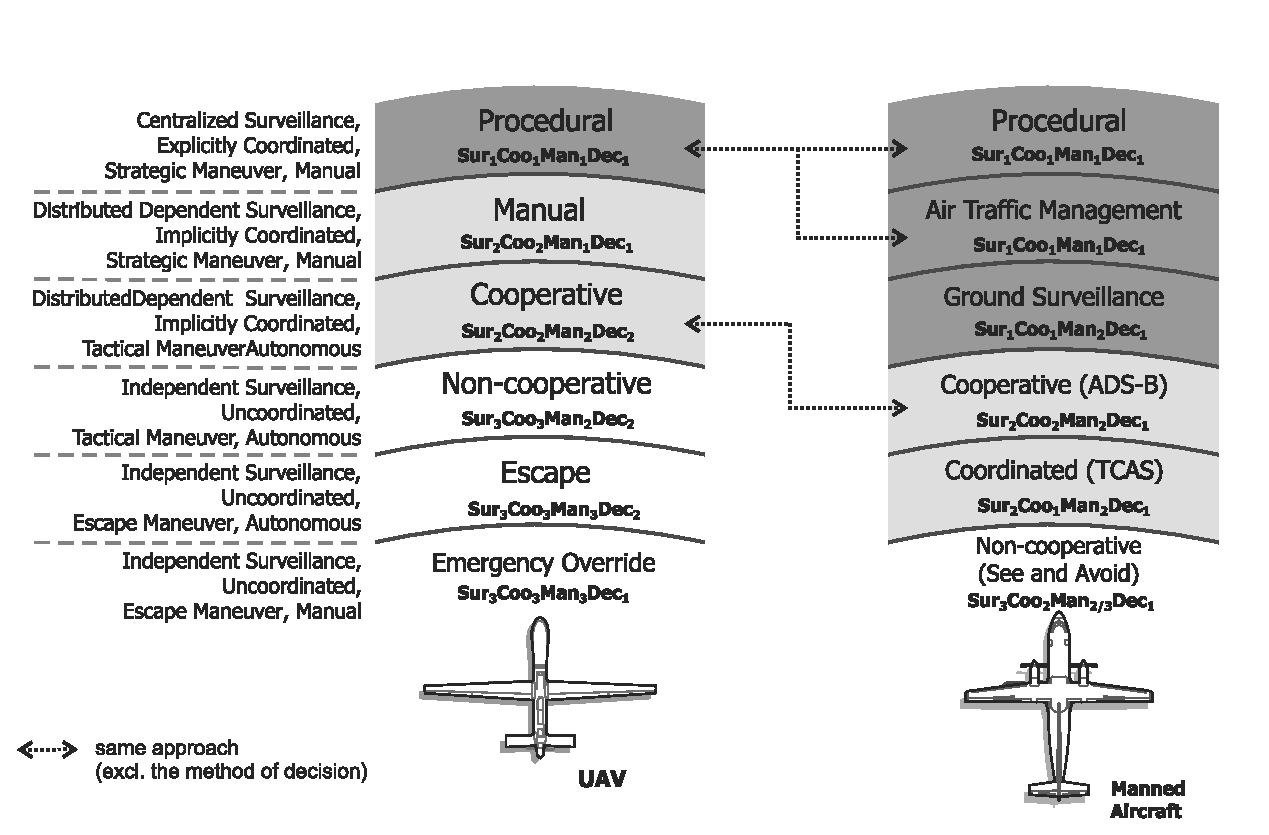
\includegraphics[width=0.8\textwidth]{\TheDir Figures/LayerofSafetyComp}
 	\caption{The novel architecture, presented as layers of safety for UAVs operation, and compared with manned-flight's\cite{Dalamagkidis:09}}
 	\label{f:LayerofSafetyComp}
 \end{figure}
 
%\subsubsection{Comparison with Manned-Flight Architecture}
Figure~\ref{f:LayerofSafetyComp} also presents a direct comparison between the new UAV CD\&R architecture and that of manned-flight. The latter is shown in the figure with the notation of method combinations used in each of its layers. Since an autonomous decision is not common in regulated manned-flight, this group of methods is excluded in this comparison.

Regarding the method combinations, for manned-flight, the two outer-most layers use the same approach of CD\&R as the Procedural Layer of the UAV. For manned-flight, these two layers are differentiated by the phase of flight in which the approach is implemented, i.e., before and during the flight. For UAVs, however, it was established before that this kind of approach is more practical to be done before the flight, due to the limitation on the centralized-dependent surveillance for UAVs. Manned flight, on the other hand, has a well-established centralized-dependent surveillance infrastructure, that can support the first three layers of safety. 

The approach used in UAVs Manual layer does not exist in manned-flight, since every rerouting (strategic maneuver) operation has to be reported to, and approved by the respective ground station, hence, a centralized dependent surveillance. In UAVs, the manual rerouting relying only on distributed-dependent surveillance, without a ground station approval, can be allowed for a short and event-driven flight like media reporting. The new route, however, should still be reported to the airspace authority by the ground operator. \cite{barfield:00}

The Cooperative layer, in both unmanned and manned-flight, uses a similar approach; an implicitly-coordinated tactical maneuver for avoidance using data from distributed-dependent surveillance. Hence, this layer is the key in the unmanned-manned flight interaction in the same airspace. A similar data protocol can be applied in the surveillance, e.g., consisting of GPS data, types, and intention. The implicit coordination can incorporate a priority rule, such as applied in VFR\cite{FAR:91} or the three laws of a \textit{Flyborg} presented in Ref.~\cite{barfield:00}. 

For manned-flight, the Coordinated layer comes after the Cooperative layer, as shown in Figure~\ref{f:LayerofSafetyComp}, as well as presented in Ref.\cite{Dalamagkidis:09}. This order actually opposes the reasoning made before, that an explicitly-coordinated avoidance should be applied before the implicitly one. The order is mainly based on the fact that the ADS-B system has a greater range than TCAS. Still, a longer range for avoidance should be more suitable for an explicit coordination. This issue is one reason to proceed with the replacement from TCAS to ADS-B, as planned in the future. %NextGen and Cesar. --> need reference But in near airport is questanable. It close, but it its explicit centralized.

The Non-cooperative layer in both unmanned and manned flight use different coordination methods. In manned flight, rules are used to enforce some type of coordination between vehicles. Therefore the avoidance always assumes that the obstacle will cooperatively obey the respected rules. This assumption is possible in conventional air traffic management, where there is only a tiny chance of encountering dangerous rogue obstacles. Even when the Cooperative layer is penetrated, one pilot can still trust that the pilot in the other aircraft has a good judgment to avoid collision while obeying the rules. In UAV flights, however, an obstacle intrusion into the Non-cooperative layer most likely means that the obstacle is rogue or has a failure in its CD\&R system, and cannot be expected to follow any rules. Therefore an uncoordinated avoidance is preferable so a UAV, which has to take into account every possible risk of collision, can avoid without being restricted to the rules. %uncoordinated menas ownship can move freely, because the otehr also wont follow

As it can be observed in Figure~\ref{f:LayerofSafetyComp}, the See and Avoid layer in manned flight can apply to two possible types of maneuver, i.e., either tactical or escape. Even though it is highly improbable, a pilot can conduct an escape during a conflict, such as turning back to the airport of departure, based on his own judgment of the situation. Hence, part of this layer is similar to the approach used in the unmanned flight Escape layer. The Emergency Override layer, on the other hand, specifically exists for UAV flights, to avoid further damage to the environment. Regulated manned-flight does not incorporate such safety layer, especially since an external pilot cannot override it. 


\subsection{Approaches Availability}
Several existing approaches for Conflict Detection and Resolution, for manned and unmanned vehicle, can be found in literature. Some of them, however, mismatch with the approaches in the architecture. Table~\ref{t:SurvivedApproaches} shows the matched and mismatched approaches that were found. The literature includes the 20 most cited and relevant papers using the keywords:\textbf{\textit{Avoidance + UAV}}\footnotemark[5]. `Avoidance' is used as a keyword since research in the UAV domain commonly used the term `collision avoidance' instead of `Conflict Detection and Resolution', which is actually a more common term in airspace management. 
This table is in the order of the combinations from Figure~\ref{f:Combination}, but omits some rows of combination that do not have any examples in literature. It should be noted that the classification of approaches is strictly based on the demonstration shown in each reference, whether by simulations or by real experiments. The potential extension of application of each approach, which can cover more than one class in Table~\ref{t:SurvivedApproaches}, is beyond the scope of this paper.\footnotetext[5]{Scopus search TITLE-ABS-KEY (avoidance uav), accessed March 2015, http://www.scopus.com/}

\begin{table}[h]
 \begin{center}
%  \begin{threeparttable}
   \caption{Existing and/or suitable combinations of methods for UAVs in civil airspace }
   \begin{tabular}{lccccl}
   \hline  \multicolumn{4}{c}{Combination} &  Designation & Examples  \\ \hline \hline%\textbf{Sur$_3$Coo$_2$Act$_2$Dec$_1$} 
   %Surv.  & Coor.  & Acti.  & Deci. &   & \\ 
        \textbf{Sur}$_1$ & \textbf{Coo}$_1$ & \textbf{Act}$_1$  & \textbf{Dec}$_1$ & Procedural & Ref. \cite{Yang:02}\tnote{\dag}, \cite{Beard:02}, \cite{Nikolos:03}\tnote{\dag}, \cite{Kaminer:06},  \cite{Borrelli:06}, \cite{Duan:09}\tnote{\dag}, \cite{Cummings:10} \tnote{\dag}\\
      %  \textbf{Sur}$_1$ & \textbf{Coo}$_1$ & \textbf{Act}$_1$  & \textbf{Dec}$_2$ & - & \\ 
      % \textbf{Sur}$_1$ & \textbf{Coo}$_1$ & \textbf{Act}$_2$  & \textbf{Dec}$_1$ & - & Ref.\\
        \textbf{Sur}$_1$ & \textbf{Coo}$_1$ & \textbf{Act}$_2$  & \textbf{Dec}$_2$ & - & Ref.~\cite{Huang:14}\tnote{\ddag}\\
      %  \textbf{Sur}$_1$ & \textbf{Coo}$_1$ & \textbf{Act}$_3$  & \textbf{Dec}$_1$ & & Ref. \\
      %  \textbf{Sur}$_1$ & \textbf{Coo}$_1$ & \textbf{Act}$_3$  & \textbf{Dec}$_2$ & & Ref. \\
      %  \textbf{Sur}$_1$ & \textbf{Coo}$_2$ & \textbf{Act}$_1$  & \textbf{Dec}$_1$ & & Ref. \\
      %  \textbf{Sur}$_1$ & \textbf{Coo}$_2$ & \textbf{Act}$_1$  & \textbf{Dec}$_2$ & - & Ref. \\ %jadi kosong?
      %  \textbf{Sur}$_1$ & \textbf{Coo}$_2$ & \textbf{Act}$_2$  & \textbf{Dec}$_1$ & & \\
        \textbf{Sur}$_1$ & \textbf{Coo}$_2$ & \textbf{Act}$_2$  & \textbf{Dec}$_2$ & & Ref. \cite{Liu:14}\tnote{\ddag} \\
      %  \textbf{Sur}$_1$ & \textbf{Coo}$_2$ & \textbf{Act}$_3$  & \textbf{Dec}$_1$ & - & Ref.  \\
        \textbf{Sur}$_1$ & \textbf{Coo}$_2$ & \textbf{Act}$_3$  & \textbf{Dec}$_2$ & & Ref. \cite{Ding:12} \\
      %  \textbf{Sur}$_1$ & \textbf{Coo}$_3$ & \textbf{Act}$_1$  & \textbf{Dec}$_1$ & & Ref. \\
      %  \textbf{Sur}$_1$ & \textbf{Coo}$_3$ & \textbf{Act}$_1$  & \textbf{Dec}$_2$ & & Ref. \\
      %  \textbf{Sur}$_1$ & \textbf{Coo}$_3$ & \textbf{Act}$_2$  & \textbf{Dec}$_1$ & & Ref. \\
      %  \textbf{Sur}$_1$ & \textbf{Coo}$_3$ & \textbf{Act}$_2$  & \textbf{Dec}$_2$ & & Ref. \\
      %  \textbf{Sur}$_1$ & \textbf{Coo}$_3$ & \textbf{Act}$_3$  & \textbf{Dec}$_1$ & & Ref. \\
        \textbf{Sur}$_1$ & \textbf{Coo}$_3$ & \textbf{Act}$_3$  & \textbf{Dec}$_2$ & - & Ref. \cite{Teo:04}\\
      %  \textbf{Sur}$_2$ & \textbf{Coo}$_1$ & \textbf{Act}$_1$  & \textbf{Dec}$_1$ & & Ref. \\
        \textbf{Sur}$_2$ & \textbf{Coo}$_1$ & \textbf{Act}$_1$  & \textbf{Dec}$_2$ & - & Ref.~\cite{Beard:02} and \cite{Duan:09}\tnote{\dag} \\
      % \textbf{Sur}$_2$ & \textbf{Coo}$_1$ & \textbf{Act}$_2$  & \textbf{Dec}$_1$ & & Ref. \\
        \textbf{Sur}$_2$ & \textbf{Coo}$_1$ & \textbf{Act}$_2$  & \textbf{Dec}$_2$ & - & Ref.  \cite{Richards:03}, \cite{Chipalkatty:12}\tnote{\ddag}, and \cite{Hurley:13}\tnote{\dag}  \\
      %  \textbf{Sur}$_2$ & \textbf{Coo}$_1$ & \textbf{Act}$_3$  & \textbf{Dec}$_1$ & Ref. \\
      %  \textbf{Sur}$_2$ & \textbf{Coo}$_1$ & \textbf{Act}$_3$  & \textbf{Dec}$_2$ & Ref. \\
        \textbf{Sur}$_2$ & \textbf{Coo}$_2$ & \textbf{Act}$_1$  & \textbf{Dec}$_1$ & Manual & -\\ 
      %  \textbf{Sur}$_2$ & \textbf{Coo}$_2$ & \textbf{Act}$_1$  & \textbf{Dec}$_2$ & & Ref. \cite{Nikolos:03}\\
       \textbf{Sur}$_2$ & \textbf{Coo}$_2$ & \textbf{Act}$_2$  & \textbf{Dec}$_1$ & - & Ref. \cite{Hoekstra:02}\tnote{\ddag}, \cite{Hoekstra:00}\tnote{\ddag}, \cite{Ellerbroek:11}\tnote{\ddag}, and \cite{Ellerbroek:13}\tnote{\ddag}\\
        \textbf{Sur}$_2$ & \textbf{Coo}$_2$ & \textbf{Act}$_2$  & \textbf{Dec}$_2$ & Cooperative & Ref. \cite{Paielli:03}, \cite{Richards:04}, \cite{Park:08}, \cite{Paul:08}, \cite{Mujumdar:11}, \cite{Prevost:11},  \cite{Yoo:11},  and \cite{Jenie:13b} \\
       \textbf{Sur}$_2$ & \textbf{Coo}$_2$ & \textbf{Act}$_3$  & \textbf{Dec}$_1$ & - & Ref. \cite{LeTallec:05}, \cite{Zeitlin:07}, and \cite{Kochenderfer:12}\tnote{\ddag}\\
      %  \textbf{Sur}$_2$ & \textbf{Coo}$_2$ & \textbf{Act}$_3$  & \textbf{Dec}$_2$ & & Ref. \\
     %   \textbf{Sur}$_2$ & \textbf{Coo}$_3$ & \textbf{Act}$_1$  & \textbf{Dec}$_1$ & & Ref. \\
     %   \textbf{Sur}$_2$ & \textbf{Coo}$_3$ & \textbf{Act}$_1$  & \textbf{Dec}$_2$ & & Ref. \\
      %  \textbf{Sur}$_2$ & \textbf{Coo}$_3$ & \textbf{Act}$_2$  & \textbf{Dec}$_1$ & & Ref. \\
      %\textbf{Sur}$_2$ & \textbf{Coo}$_3$ & \textbf{Act}$_2$  & \textbf{Dec}$_2$ & - & Ref.  \\
        \textbf{Sur}$_2$ & \textbf{Coo}$_3$ & \textbf{Act}$_3$  & \textbf{Dec}$_1$ & - & Ref. \cite{Winder:99}\\
      %  \textbf{Sur}$_2$ & \textbf{Coo}$_3$ & \textbf{Act}$_3$  & \textbf{Dec}$_2$ & & Ref. \\ 
      %  \textbf{Sur}$_3$ & \textbf{Coo}$_1$ & \textbf{Act}$_1$  & \textbf{Dec}$_1$ & & Ref. \\
        \textbf{Sur}$_3$ & \textbf{Coo}$_1$ & \textbf{Act}$_1$  & \textbf{Dec}$_2$ & - & Ref.  \cite{Kelly:06}\tnote{\dag}, \cite{Langelaan:07}\tnote{\dag}, \cite{Obermeyer:12}\tnote{\dag}, and \cite{Chowdhary:12}\tnote{\dag}\\
      %  \textbf{Sur}$_3$ & \textbf{Coo}$_1$ & \textbf{Act}$_2$  & \textbf{Dec}$_1$ & Ref. \\
        \textbf{Sur}$_3$ & \textbf{Coo}$_1$ & \textbf{Act}$_2$  & \textbf{Dec}$_2$ & - & Ref. \cite{Netter:02}\tnote{\dag}, \cite{Nikolos:03}\tnote{\dag}, \cite{Yang:04}\tnote{\dag}, \cite{McGee:05}\tnote{\dag}, \cite{Patel:11}\tnote{\dag}, \cite{Hrabar:11}\tnote{\dag}, and \cite{Jung:13}\tnote{\dag} \\
        \textbf{Sur}$_3$ & \textbf{Coo}$_1$ & \textbf{Act}$_3$  & \textbf{Dec}$_1$ & - & Ref. \cite{Lam:09b}\tnote{\dag}\\
        \textbf{Sur}$_3$ & \textbf{Coo}$_1$ & \textbf{Act}$_3$  & \textbf{Dec}$_2$ & - & Ref. \cite{Muratet:05}\tnote{\dag}, \cite{Beyeler:09}\tnote{\dag}, \cite{Bouabdallah:07}\tnote{\dag}, \cite{deCroon:11}\tnote{\dag}, \cite{deCroon:12}\tnote{\dag}, and \cite{Muller:14}\tnote{\dag} \\
      %  \textbf{Sur}$_3$ & \textbf{Coo}$_2$ & \textbf{Act}$_1$  & \textbf{Dec}$_1$ & & Ref. \\
      %  \textbf{Sur}$_3$ & \textbf{Coo}$_2$ & \textbf{Act}$_1$  & \textbf{Dec}$_2$ & & Ref. \\
      %  \textbf{Sur}$_3$ & \textbf{Coo}$_2$ & \textbf{Act}$_2$  & \textbf{Dec}$_1$ & & Ref. \\
        \textbf{Sur}$_3$ & \textbf{Coo}$_2$ & \textbf{Act}$_2$  & \textbf{Dec}$_2$ & - & Ref. \cite{Kitamura:95}, \cite{Yang:04}, \cite{Wang:07}, \cite{Fasano:08}, \cite{Prevost:11}, \cite{Choi:13}, \cite{Klaus:13}, and \cite{Schmitt:14} \\
      %  \textbf{Sur}$_3$ & \textbf{Coo}$_2$ & \textbf{Act}$_3$  & \textbf{Dec}$_1$ & & Ref. \\
      %  \textbf{Sur}$_3$ & \textbf{Coo}$_2$ & \textbf{Act}$_3$  & \textbf{Dec}$_2$ & & Ref. \\
      %  \textbf{Sur}$_3$ & \textbf{Coo}$_3$ & \textbf{Act}$_1$  & \textbf{Dec}$_1$ & & Ref. \\
      %  \textbf{Sur}$_3$ & \textbf{Coo}$_3$ & \textbf{Act}$_1$  & \textbf{Dec}$_2$ & & Ref. \\
      %  \textbf{Sur}$_3$ & \textbf{Coo}$_3$ & \textbf{Act}$_2$  & \textbf{Dec}$_1$ & & Ref. \\
        \textbf{Sur}$_3$ & \textbf{Coo}$_3$ & \textbf{Act}$_2$  & \textbf{Dec}$_2$ & Non-cooperative & Ref.~\cite{Rathbun:02} \\
        \textbf{Sur}$_3$ & \textbf{Coo}$_3$ & \textbf{Act}$_3$  & \textbf{Dec}$_1$ & Emergency Override & - \\  
        \textbf{Sur}$_3$ & \textbf{Coo}$_3$ & \textbf{Act}$_3$  & \textbf{Dec}$_2$ & Escape & -  \\ 
       \hline 
   \end{tabular} 
   \begin{tablenotes}
    \item[\dag] Indoor application, against static obstacles.
    \item[\ddag] Manned-flight applications
    \end{tablenotes}
  \label{t:SurvivedApproaches}
%  \end{threeparttable}
 \end{center}
\end{table}

Table~\ref{t:SurvivedApproaches} shows that most approaches in the 54 references do not comply with the layers of the proposed architecture. The Procedural and the Cooperative layer seem to be popular that they have more than five representatives. One reference can be found that uses the Non-Cooperative approach. On the other hand, examples for approaches in the Manual, Escape, and Emergency Override Layers were not found in literature.

The combination of centralized-dependent surveillance and the explicit coordination is widely used in Path Planning problems. The Global Path Planning in particular fits well with the Procedural Layer, (\textbf{Sur$_1$Coo$_1$Act$_1$Dec$_1$}), since it relies on predetermined map of the obstacles. This paper classified the approach to be manually decided by assumption that the algorithm is triggered by the operator decision at the beginning of the mission.

The Manual Layer (\textbf{Sur$_2$Coo$_2$Act$_1$Dec$_1$}) does not have any example in literature. The closest approach probably is the Local Path Planner, such as used in Ref.~\cite{Beard:02} and \cite{Duan:09}. These references show the extension of Global Path Planner by giving the vehicle ability to conduct a re-planning when it detects obstacles that are not listed in its predetermined map before. The only difference with the approach in Manual Layer is the autonomous assumption, which can be easily change to manual decision in deciding the new waypoints.

Many examples of references match with the approach in the Cooperative Layer (\textbf{Sur$_2$Coo$_2$Act$_2$Dec$_2$}). The reason of this popularity is probably because most research considers the optimized autonomous system to be the cutting edge technology for UAV avoidance. The number of examples in this layer can be even larger if the research in manned-flight approaches, in the (\textbf{Sur$_2$Coo$_2$Act$_2$Dec$_1$}) row, are also included by neglecting the decision method.

The approach in Non-cooperative Layer, a combination of methods that are commonly used in the UAV avoidance research (\textbf{Sur$_3$Coo$_3$Act$_2$Dec$_2$}), is supposed to have a number of examples. This, however, does not seems to be the case, where only one paper falls into this layer, as shown in table~\ref{t:SurvivedApproaches}. The reason is that while the papers intended to be an autonomous uncoordinated tactical avoidance relying on independent surveillances (on-board sensors), they use the assumption of non-maneuvering obstacles. Hence, the approach in these studies is considered to be an implicitly coordinated avoidance in the proposed taxonomy. Ref.~\cite{Rathbun:02} stands out in literature as being the only example of an autonomous tactical maneuver for avoidance from maneuvering obstacles, while using independent surveillance. Other examples on uncoordinated escape approaches for avoidance are also shown in Ref.~\cite{Teo:04} and \cite{Winder:99}.

While an exact example for the Escape Layer (\textbf{Sur$_3$Coo$_3$Act$_3$Dec$_2$}) is not found in literature, many studies used the concept of an open-loop input that generates escape avoidance. However, these studies focus on approaches to handle static obstacles and, hence, included as an explicit coordinated avoidance, resided in the (\textbf{Sur$_3$Coo$_1$Act$_3$Dec$_1$}) and (\textbf{Sur$_3$Coo$_1$Act$_3$Dec$_2$}) rows. The work in Ref.~\cite{Teo:04} with its Emergency Escape Maneuver (EEM) comes close for the Escape Layer. However, in the approach demonstration, it still relies on a centralized dependent surveillance at the ground.

No approach exists in the literature that can be fitted into the Emergency Override layer. The work in Ref.~\cite{Lam:09a} is probably the closest one for the layer. The approach of providing a haptic feedback might be extended to handle dynamic obstacles, and used to inform the ground operator about the flight conditions.

\section{Architecture Implementation}
The implementation of the defined architecture depends on the mission of each UAV. In one particular mission some layers in the architecture might become unnecessary while in others they might be important. Some of the layers can impose requirements to the CD\&R system and infrastructure. This section presents a general implementation of the architecture for UAV operations in the civil airspace, followed by a few examples for prospective UAV operations, given in Table~\ref{t:Category}, which are based on the work Ref.~\cite{degarmo:04} with a few additions. This research limits itself to these examples of UAV missions, without ruling out others that might already exist.

\begin{figure}[h]
	\centering
	\includegraphics[width=0.8\linewidth]{\TheDir Figures/Prospectives}
	\caption{Prospective use of UAVs in Civil Airspace, adapted from Ref.~\cite{degarmo:04}. Numbers are referred to Table~\ref{t:Category}}
	\label{f:Prospectives}
\end{figure}

\begin{table}
 \begin{center}
%  \begin{threeparttable}
   \caption{Prospective UAVs operation in the civil airspace, partly adapted from Ref.\cite{degarmo:04}}
  \begin{tabular}{clccccc}
  \hline  
  No & Mission  &  Operational & Cruising  & Cruising & Maximum & Endurance\\ 
   & & Weight &  Speed & Altitude  & Range &     \\
  \hline\hline
  1 & Telecommunication Airship\cite{degarmo:04,Colozza:03,Colozza:05}  & 20 ton & n/a & 20 km & n/a & 1 year\\ %HALE --> above the airspace, long endurance. if hig altitude, count as rural? except if we are counting on the information, but here we focus on sfaety only, not security
  2 & High-Altitude Imagery\cite{degarmo:04,Romeo:04}  & 800 kg & 96 km/h & 18 km & 3 km & 9 months\\  % HALE 
  3 & Border Patrol\cite{degarmo:04,Girard:04}  &  25 kg & 50 km/h & $<$ 6 km & 25 km & n/a \\  %Medium Altitude, medium endurance, rural
  4 & Maritime Surveillance\cite{degarmo:04,Meester:13} &  20 kg & 133 km/h & $<$ 6 km & 500 km  & 5 hr  \\  %Medium Altitude, medium endurance, rural MAMER
  5 & Environmental Sensing\cite{degarmo:04,Casbeer:05}  &  25 kg & 50 km/h & $<$ 6 km & 25 km & 40 min. \\ %%Medium Altitude, medium endurance, rural MAMER 
  6 & Media and Traffic Reporting\cite{degarmo:04,Frew:04}  & 10 kg & 60 km/h & $<$1.5 km & 25 km & 40 min.  \\  %Medium Altitude, short endurance, urban MASEU
  7 & Law Enforcement\cite{degarmo:04,Herwitz:04} &  25 kg & 10 km/h & $<$ 120 m & n/a & 8 hr.  \\ %Low Altitude, short endurance, urban LASEU
  8 & Delivery Service\cite{D'Andrea:14} & $<$25 kg & 80 km/h & $<$ 120 m & 25 km & 30 min. \\  %Low Altitude, Medium endurance, urban/rural LAMEU/R
  \hline 
  \end{tabular} 
%   \begin{tablenotes}
%   \end{tablenotes}
  \label{t:Category}
%  \end{threeparttable}
 \end{center}
\end{table}

The implementation is discussed under the assumption that UAVs are already integrated in the airspace system, as depicted in Figure~\ref{f:Prospectives}. The aerodrome airspace (class B, C and D), however, remains highly restricted. Class A airspace is also restricted for the main operation of any UAV, except for short periods, like climbing for a High-Altitude-Long-Endurance (HALE) UAV. Class E becomes the airspace with the highest risk since both (small) manned-aircraft, as well as UAVs, are flying in there. The prospective UAV operations in Table~\ref{t:Category} are grouped into three types of UAVs, i.e., HALE, Rural Surveillance, and Urban Low Altitude UAVs.

\subsection{General Implementation}

The layers of safety are generally implemented as follows. First, before the flight is even conducted, the operator seeks approval for the flight-plan for the UAV mission. This activity is represented by the Procedural Layer. The aim, here, is to avoid any unnecessary conflict with other traffic, static obstacles, or bad weather. This is done with a centralized surveillance such as an Air Traffic Control (ATC) station, or other network stations. The operator, therefore, is responsible for giving the designated flight plan back to the center. This layer filters any unnecessary conflicts from the UAV operation.

After departure, the UAV relies first on its dependent surveillance system, which, with the current technology, could be either the ADS-B, or FLARM\footnotemark[4]. The system detects other vehicles, manned and unmanned, early enough to send the updated traffic data to the ground, and conduct a manually decided strategic maneuver. This is the Manual layer of the architecture. The implicit-coordination in this layer can be a simple rule like, for example, not to bother the existing traffic (first-come-first-served). This layer will avoid any cooperative obstacles that are detected early enough to select other alternatives.\footnotetext[4]{-. "FLARM: What Is It", -, accessed September 2014, http://www.gliderpilot.org/Flarm-WhatIsIt}

In cases where a strategic maneuver is not preferable due to mission importance like saving fuel, the UAV can choose to avoid with a tactical maneuver, implementing the Cooperative Layer. Another example is when, due to some failures, the cooperative counterpart is not detected soon enough to change several waypoints. The avoidance in this layer is conducted autonomously due to the assumed lack of situational awareness of the ground operator. Implicit rules, such as an adaptation of the manned-flight Visual Flight Rules (VFR)\cite{FAR:91}, can be applied to simplify the resolution. At this point, all conflicts with normal manned-aircraft are resolved. 

By using independent-surveillance, the last three layers are actually substitutes to the `see and avoid' layer in manned flight. The Non-cooperative Layer intends to avoid obstacles that are able to penetrate through the first three layers, which can be non-cooperative vehicles, or cooperative vehicles with some system failures. The uncoordinated avoidance should be the choice either way to take account of all the risk. The type of independent surveillance will determine the distance where this layer is applied. In this layer, every conflict with normal aircraft, manned or unmanned, is resolved.

The Escape Layer aims to avoid any remaining non-cooperative obstacles that are hard to detect within sufficient range for a tactical maneuver. With the advancement of independent surveillance technology, however, the probability to encounter these obstacles is small. An escape should be aggressive using the maximum ability of the vehicle to avoid collision. There will only be a very short distance left for the calculation process, so a predefined sure-escape maneuver is preferable. Therefore, the vehicle's maneuverability should be the deciding factor in implementing the layer. The work of Ref.~\cite{barfield:00}, for example, sets the time of 1.5 second-to-collision to start escaping.

Due to various unexpected situations, penetrations through all the five previous layers are still possible. For example, there might be a failure in the autonomous CD\&R system, or an unpredicted acceleration from the counterpart. In these situations, the operator on the ground can take over and conduct avoidance sooner, compared to the autonomous processes. This also applies in adverse situations where a collision has occurred, but only partially damages the own-ship. Operators should have an emergency override to prevent any further damage, including, for example, preventing the crippled UAV to fall into a populated area.

\subsection{High Altitude Long Endurance (HALE) UAV}
Two UAV types and missions in Table~\ref{t:Category} are included in the HALE -UAV category, i.e., the Stratospheric Telecommunications Airship\cite{Colozza:03,Colozza:05} and High-Altitude Imagery\cite{Romeo:04}. Both of them operate at altitudes over 20 km, higher than the class A airspace where commercial aircraft commonly cruise. Both of them are most likely to have low maneuverability, considering their type, i.e., an airship and a very-high aspect-ratio fixed wing. This will induce some difficulty in applying a tactical or an escape maneuver. The vehicle will therefore rely more on strategic maneuver for avoidance.

A HALE -UAV will depart from a rural base, and directly climb to its operational altitude. This short climb phase might involve some encounters with various other UAVs and small manned-aircraft in the class E airspace, and with big commercial aircraft in the class A-airspace as well. The safest way for the operation would be to fly in a secluded area away from any manned flight. In cases where it cannot be fully secluded, however, the possibility of encounters with manned-flight will require the UAV to communicate its flight-plan with an Air Traffic Control (ATC) to obtain some level of clearance. A HALE-UAV area of operation, the upper class-E airspace, on the other hand, can almost be considered as physically secluded from other UAV and manned aircraft. 

For the dependent surveillance system, which in the current technology can be the ADS-B\cite{McCallie:11}, or the FLARM, the manned-flight's ADS-B is more preferable due to its longer range of detection (until 185 km) compared to the 5 km the FLARM can offer. The long range of detection allows for more avoidance possibilities, especially for a vehicle with low maneuverability. A TCAS is also an option to be more compatible with the current manned-flight system, but will add an extra 10 kg.

For the independent surveillance, the most popular choice currently is a visual light camera system, which has detection range of up to 10 km. However, especially for a large airship, a system with further detection range like the airborne RADAR is also a choice. The system will be suitable for detecting a metal manned-flight, the most important vehicle to be avoided, with a detection range of 15 km. The weight of such system, however, reaches 25 kg, which can significantly reduce the payload capacity. Current research that is working on airborne RADAR miniaturization\cite{Moses:14}  might open other possibilities in the near future. 

\subsection{Rural Surveillance UAV}
The Border Patrol\cite{Girard:04}, Maritime Surveillance\cite{Meester:13}, and Environmental Sensing UAV \cite{Casbeer:05} are included in Tactical Surveillance UAVs. Those three operate in the class E airspace under 18,000 feet, where there is a possibility to encounter other similar types of UAVs. Weighing around 25 kg, this type cannot carry a heavy surveillance system such as the manned-flight version of the ADS-B\cite{McCallie:11}. Instead, the FLARM , that is less than 500 grams, is more preferable. Different from the HALE, most of these UAVs have high maneuverability, thus can rely more on tactical maneuvers for avoidance. There will also be more variation in aircraft type, which ranges from a hand launched fixed-wing to a vertical take-off rotary wing. Considering its medium endurance and area of operation, the UAV will depart from a rural base and operates away from populated areas.

Similar to the HALE, this type of UAV needs to communicate its flight plan with an ATC as the centralized dependent surveillance. The clearance should consider small manned aircraft, and any registered UAV flying in the area. The clearance, however, might not be mandatory, since these UAVs are also meant for event-based or emergency operation, for example, a Maritime Surveillance UAV flight to survey a tanker accident. Therefore, the avoidance should be relying more on the other two surveillance systems. Manual decision will have a small role, because of the short range of detection the FLARM can provide for the Manual Layer. Therefore, in most of its operation the UAV will implement directly the third layer, and avoid obstacles using an implicitly coordinated tactical maneuver. Rules such as the VFR are used for the avoidance, especially in the encounter with other UAVs. In emergency situations such as a search and rescue operation, however, the UAV might have the highest priority among others and, thus, override the VFR. 

A light-weight camera system can be used for its independent surveillance. The UAV developer can also consider combining the surveillance system with the camera the UAV uses for its main task. The distance to start the Non-cooperative Layer, however, needs to be determined based on, for example, the risk imposed by a non-cooperative obstacle.

\subsection{Urban Low Altitude UAV}
The Urban Low Altitude UAV describes three of the UAVs in Table~\ref{t:Category}, including the Media and Traffic Reporting\cite{Frew:04}, Delivery Service\cite{D'Andrea:14}, and Tactical Law Enforcement UAVs\cite{Herwitz:04}. These UAVs operate in low altitude below 1.5 km, and mostly above urban areas like cities, inside the class-G airspace. The UAVs are commonly electric-powered rotary wings, which are able to hover and perform other narrow-spaced maneuvers. This type of UAV probably has the largest number of interested companies, hoping to be able to fly it from the roof of their buildings. The flight, therefore, needs to take account of static obstacles, like towers and buildings, more than the HALE or the Rural Surveillance UAV. During its low altitude and short period of flight, it is almost impossible for it to encounter manned flight. The operation is secluded in the city area, and probably its greatest dynamic threat is birds and other UAVs. Flight into the airport aerodrome should be highly restricted.

The procedural layer implementation will require many infrastructure developments. Instead of an ATC, the centralized-dependent-surveillance for this layer requires a new infrastructure or establishment among the urban operators, and should also be accessible for the authorities and general public, i.e., by using the Internet. On departure, a UAV needs to match the schedule in some common departure point establishment in the area. A Delivery UAV may require some sort of a clearance or permission from a common end point. Data from these establishment should also include information about buildings and towers and other landmarks in proximity. 

FLARM is a definite choice for the distributed-dependent surveillance in the current technology. A special type of surveillance can be made for urban applications, along with their special implicit rules. 

For the independent surveillance, a camera system is an option, but other types of sensors are also being developed in a rapid phase that can be lighter and lower in power consumption. The detection range requirements can be short due to the high maneuverability of the UAV. Special precaution, like a parachute system, should be made in the Emergency Override layer, to avoid falling in a populated area or crashing into a building.

\section{Conclusion}
The paper elaborated approaches for an Unmanned Aerial Vehicle (UAV) Conflict Detection and Resolution (CD\&R) system from literatures and defines a taxonomy of methods. It is shown that the approaches can be viewed as a generic combination of choices in method of surveillance, coordination, maneuver and decision. In the context of UAV integration into the civil airspace system, some of these generic approaches are appropriate and some are not. 

A novel architecture for UAV CD\&R systems is derived by arranging appropriate approaches using the fail-safe concept. This architecture consists of six layers of safety, which are, from the outermost, the Procedural, the Manual, the Cooperative, the Non-cooperative, the Escape, and the Emergency Override Layer. Some of these layers do not have adequate number of examples in literature, suggesting some new research areas that should be a focus to speed up the UAV integration.

Each layer in the architecture can be a guideline for requirements in the systems and infrastructures of UAV CD\&R for an integrated operation in the civil airspace. The requirements might differ across various UAV, since some layers might be less significant than the others depending on the specific type and mission. Thresholds for each of the layers need to be defined, specifically for each mission, for the practical use of the architecture to support UAV integration into the civil airspace system.

